
\setchapterpreamble[u]{\margintoc}
\chapter{Nuclear spin control via microwaves}
\labch{nuclea_spin_control}

In this chapter we describe the techniques used to coherently controlling a nuclear spin that is strongly coupled to an \Er ion. 

\section{Driving a nuclear spin-1/2}
\labsec{driving_nuclear_spin_half}

If one wishes to drive the state of a nuclear spin, the most straightforward way is to apply a radiofrequency (rf) pulse resonant with a nuclear spin transition. However, as detailed in \refsec{rabi_oscillations_theory}, in our setup the superconducting resonator acts as a narrow band-pass filter centered around $\omega_r\approx7.7$~GHz. Consequently, all rf drives applied to the sample will be reflected from the resonator and direct driving of a nuclear spin becomes impossible.

In order to find an alternative driving scheme, we now consider the Hamiltonian of an \Er spin-1/2 coupled via hyperfine interaction to a nuclear spin-1/2 while under a magnetic field $B_0$. As described in \refch{electron_nuclear_interaction}, the Hamiltonian under the secular approximation can be written as

\begin{equation}
    \cH{} = \omega_S \hat{S}_z + \omega_I \hat{I}_z + A_\parallel \hat{S}_z \hat{I}_z + A_\perp \hat{S}_z \hat{I}_x.
\end{equation}

This Hamiltonian is analytically solvable \sidecite{schweiger_principles_2001} and the nuclear and electron transition frequencies are given by

\begin{marginfigure}
    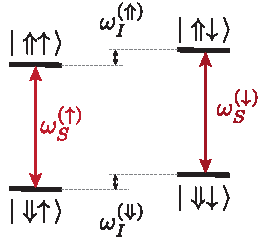
\includegraphics{chapter2/figures/energy_levels_half.pdf}
    \caption[Energy level diagram of an Er3+ coupled to a nuclear spin-1/2]{Energy level diagram of an \Er coupled to a nuclear spin-1/2.}
    \labfig{energy_levels_half}
\end{marginfigure}

\begin{align}
\begin{split}   
     \omega_I^{(\Uparrow)} &= \left(\omega_I + \frac{A_\parallel}{2}\right) \cos \eta_\alpha - \frac{A_\perp}{2} \sin \eta_\alpha, \\ 
    \omega_I^{(\Downarrow)} &= \left(\omega_I - \frac{A_\parallel}{2}\right) \cos \eta_\beta - \frac{A_\perp}{2} \sin \eta_\beta, \\ \\
    \omega_S^{(\uparrow)} &= \omega_S + \frac{1}{2} \left( \omega_I^{(\Uparrow)} - \omega_I^{(\Downarrow)} \right) \\ 
    \omega_S^{(\downarrow)} &= \omega_S - \frac{1}{2} \left( \omega_I^{(\Uparrow)} + \omega_I^{(\Downarrow)} \right) \\ \\
    \eta_{\alpha, \beta} &= \arctan{\left(\frac{-A_\perp}{A_\parallel \pm 2\omega_I}\right)}.
\end{split}    
\end{align}

where $\eta_{\alpha, \beta}$ are the mixing angles. 

In the high-field regime, $|\omega_I| \gg |A_\parallel|, |A_\perp|$, the mixing angles vanish and the eigenstates are well approximated by the uncoupled spin states $\ket{\Downarrow \uparrow}$, $\ket{\Downarrow \downarrow}$, $\ket{\Uparrow \uparrow}$, $\ket{\Uparrow \downarrow}$, as illustrated in \reffig{energy_levels_half}. Because the electron and nuclear gyromagnetic factors have opposite signs ($\omega_I < 0 < \omega_S$) the ground state has the two spins antiparallel. Under these conditions the transition energies can be approximated to

\begin{align}
\begin{split}
    \omega_I^{(\Uparrow)} = \omega_I + \frac{A_\parallel}{2}, &\qquad \omega_I^{(\Downarrow)} = \omega_I - \frac{A_\parallel}{2}, \\
    \omega_S^{(\uparrow)} = \omega_S + \frac{A_\parallel}{2}, &\qquad \omega_S^{(\downarrow)} = \omega_I - \frac{A_\parallel}{2}.
\end{split}    
\end{align}




\begin{itemize}
    \item Hamiltonian and weakly allowed transitions
    \item Matrix element calculation
    \item AC-Zeeman shift
    \item Cross-relaxation probability
\end{itemize}

\section{Stimulated Raman driving}
\labsec{raman_driving}

\begin{itemize}
    \item Principles
    \item Stimulated Raman shift
\end{itemize}

\section{High-spin generalization}
\labsec{high_spin_generalization}

\begin{itemize}
    \item New Hamiltonian
    \item Matrix elements recalculated
\end{itemize}